%% vim:tw=66:spell:wrap:ft=tex
\documentclass[%
        hyperref={%
                pdfauthor={Zakariyya Mughal},%
                pdfpagemode={None},pdfpagelayout={SinglePage}}%
        xcolor={x11names},%
]{beamer}
\usetheme{Warsaw}
\usecolortheme{crane}
\usepackage{textcomp}
\usepackage{fancyvrb}
\usepackage{changepage}
\usepackage{multicol}
%\usepackage{wasysym}
\usepackage{multimedia}
\usepackage{listings}
\newenvironment{indented}{\begin{adjustwidth}{1.5em}{}}{\end{adjustwidth}}

\usepackage{tikz}
\usetikzlibrary{snakes,arrows,shapes,automata}

\title[Unicode]{Things you (probably) didn't know about Unicode}
\author{Zaki Mughal}
\institute{University of Houston:\\CougarCS}
\date{2013 Oct 10}
\begin{document}

\frame{\titlepage}

\frame{
\centering
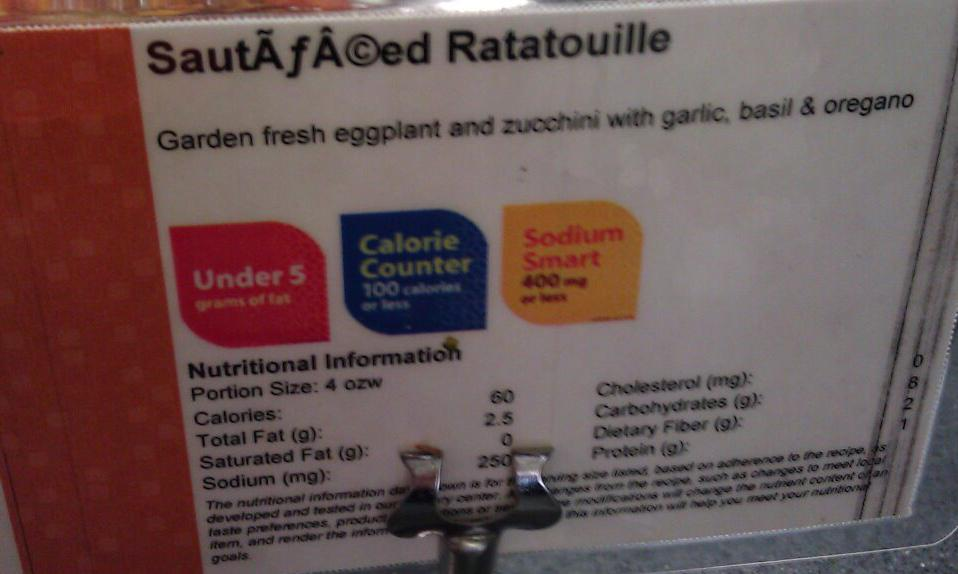
\includegraphics[width=0.8\textwidth]{gfx/mojibake.jpg}

\pause This is mojibake.
}

\begin{frame}
\frametitle{ASCII you a question}
\begin{center}
\begin{minipage}{0.5\textwidth}
\lstinputlisting{gfx/unicode.figlet}
\end{minipage}
\end{center}
\end{frame}

\begin{frame}
\begin{itemize}
\item \emph{Unicode} is a standard for encoding, representation, and text
handling. It tries to cover every character of the world's
languages.

\pause\item It stores each character as a code-point $\rightarrow$  from \texttt{U+0000}
to \texttt{U+10FFFF}. 1,114,112 code-points.
\end{itemize}
\end{frame}

\begin{frame}
\begin{itemize}
\frametitle{Myths}
\item Myth: ASCII is good enough. English is the only language used on computers.
\pause\item We're in Houston. We know this.
\pause\item I just needed to get that out of the way.
\end{itemize}
\end{frame}

\begin{frame}
\begin{itemize}
\item Myth: We're using English. We can still use plain text with good ol' ASCII.
\item Words you can't store in ASCII: r\'esum\'e, na\"{\i}ve, no\"el.
\pause\item Oh, and ASCII is actually just the characters 0 --
127. The rest (128-255) are extensions that can vary by encoding. \pause
There are many encodings.
\end{itemize}
\end{frame}

\begin{frame}
\frametitle{Myths}
\begin{itemize}
\frametitle{Myths}
\item Myth: OK, everything is in Unicode. We'll just use Unicode
\pause\item not everything is in Unicode
\pause\item You can't just \emph{use} Unicode. It's a bit harder than that\ldots
\pause\item \quad\emph{Languages are hard.} \pause In fact, anything
dealing with the real world data is \emph{hard}. See: date-time libraries.
\end{itemize}
\end{frame}

\frame{
Doing things wrong means others will have to try to
clean up your mistakes.
\pause

\centering
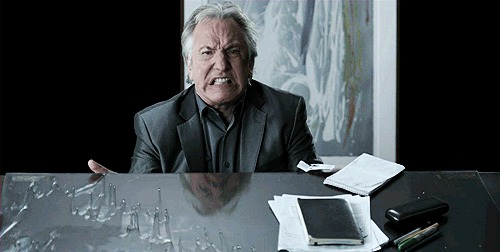
\includegraphics[width=0.9\textwidth]{gfx/alan-rickman-flip.jpg}
}

\begin{frame}
\begin{itemize}
\item You can't assume encodings.
\pause\item If you assume an encoding for any reason (ASCII,
platform-specific, English-only input), your code is broken.
\pause\item This is why you set Content-Type in your HTTP headers
or use a \texttt{<meta>} in your HTML. \pause Or you'll leave
browsers guessing. Which you don't want.
\end{itemize}
\end{frame}

\begin{frame}
\begin{itemize}
\item Characters aren't 8-bits.
\pause\item Yes, \texttt{char} in C is still 8-bits.
\pause\item A \texttt{char*} can not handle Unicode by itself.
\pause\item You need a library like International Components for
Unicode (\texttt{libicu}) \url{http://www.icu-project.org/}
\end{itemize}
\end{frame}

\begin{frame}
\frametitle{How many bits do we need then?}
\begin{itemize}
	\item UTF-32: 32-bits, uses most space
	\item UTF-16:
\end{itemize}
\end{frame}

\begin{frame}
\begin{center}
You'll need to throw away a lot of assumptions you make about text...
\end{center}
\end{frame}

\begin{frame}
\frametitle{Uppercase and lowercase}
\begin{center}
\begin{minipage}{0.9\textwidth}
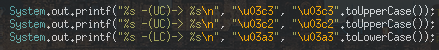
\includegraphics[width=1\textwidth]{gfx/java-uc-lc.png}
\end{minipage}
\end{center}

\bigskip

\begin{center}
\begin{minipage}{0.3\textwidth}
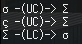
\includegraphics[width=1\textwidth]{gfx/java-uc-lc-out.png}
\end{minipage}
\end{center}
\end{frame}

\begin{frame}
You can't uppercase every letter:
\begin{itemize}
\item The German eszett (\ss) has no uppercase equivalent (well, officially)
\item If you use all-caps, you need to convert it to two letters:
gro\ss $\rightarrow$ GROSS.
\lstinputlisting{src/SS.pl}
\pause\item Yes, all-caps changes the length of the string\ldots
\end{itemize}
\end{frame}

\begin{frame}
\begin{itemize}
\item Myth: Unicode is just like ASCII but with more characters.
\item The standard also specifies algorithms, including:
\end{itemize}
\end{frame}


\begin{frame}
\begin{itemize}
\item casemapping, casefolding
\item grapheme clusters
\item normalization
\item collation
\item word- and line-breaking
\item properties database (uppercase, lowercase, letter, number, etc.)
\item bidirectional text
\item glyph variants
\end{itemize}
\end{frame}

\begin{frame}
These algorithms affect anything you have that deals with text:
\begin{itemize}
\item word wrapping
\item sorting
\item rendering
\item changing the case
\item sorting strings
\item checking if two strings are equal
\end{itemize}
\end{frame}

\begin{frame}
\begin{itemize}
\item Collation: sorting differs from language to language
\pause\item German treats `o' and `\"o' as the same letter, but
Turkish treats them as different letters.
\pause\item \texttt{strcmp} in C compares bytes. \texttt{strcoll} uses
your \emph{locale}
\item on POSIX systems, you can use \texttt{LC\_*} environment variables to set
your locale
\pause\item if you don't care about locales, you can set
\texttt{LC\_ALL="C"} and speed up some some utilities like
\texttt{sort}
\end{itemize}
\end{frame}


\end{document}
